\section{Particle Filters}
\label{particle_filters}

Gaussian filtering is a useful technique in order to perform nonlinear filtering and we have seen
the extended and unscented Kalman filtering. However, these methods do not perform well when

\begin{itemize}
\item The models are highly nonlinear
\item When the posterior distribution is significantly non-Gaussian e.g. a multimodal density
\end{itemize}


For these kinds of problems we need a different type of approximation to the posterior density. One such approach is the particle filter
method that we will discuss in this section. The idea behind this filtering technique is  to aquire point-wise
estimates, called samples, of the posterior $p(\mathbf{x}_k | \mathbf{y}_{1:k})$. Then, as the number of samples increases,
the accuracy of the approximation increases. 


\begin{framed}
\theoremstyle{remark}
\begin{remark}{}

Particle filters are also known as sequential importance resampling or sequential Monte Carlo.
The basis of these methods is an algorithm called  sequential importance sampling.
\end{remark}
\end{framed}

\section{Introduction to Particle Filtering }
\label{particle_filter_introduction}

The basic idea behind particle filtering is to use a non-parametric representation of the posterior

\begin{equation}
p(\mathbf{x}_k | \mathbf{y}_{1:k}) \approx \sum_{i=1}^N w_{k}^{(i)} \delta (\mathbf{x}_k -\mathbf{x}_{k}^{(i)})
\end{equation}

where $\mathbf{x}_{k}^{(i)}$ are particles and $w_{k}^{(i)}$ are associated weights.

We can then perform filtering by propagating $\mathbf{x}_{k}^{(i)}$ over time and
updating the weights.


\subsection{Monte Carlo sampling}
\label{monte_carlo_sampling}

Given independent samples $\mathbf{x}^{(1)}, \mathbf{x}^{(2)}, \ldots, \mathbf{x}^{(N)} \sim p(\mathbf{x})$ we can approximate

\begin{eqnarray}
E[\mathbf{g}(\mathbf{x})] \approx \frac{1}{N}\sum_{i=1}^N \mathbf{g}(\mathbf{x}^{(i)}) \\
p(\mathbf{x}) \approx \frac{1}{N}\sum_{i=1}^N \delta(\mathbf{x} - \mathbf{x}^{(i)})
\end{eqnarray}

Monte Carlo approximations have the following characteristics

\begin{itemize}
\item Non-parametric approximation to $p(\mathbf{x})$
\item Approximates all kinds of densities $p(\mathbf{x})$
\item Does not suffer from the curse of dimensionality
\end{itemize}

\begin{framed}
\theoremstyle{remark}
\begin{remark}{\textbf{Curse of Dimensionality}}

\end{remark}
\end{framed}

However, we should note that it is often difficult to generate samples from $p(\mathbf{x})$

\subsection{Importance sampling}
\label{importance_sampling}

Importance sampling can be used when it is difficult to sample from $p(\mathbf{x})$. Importance sampling generates samples
$\mathbf{x}^{(1)}, \mathbf{x}^{(2)}, \ldots, \mathbf{x}^{(N)}$ from a a proposal density $q(\mathbf{x})$. We can then set $p(\mathbf{x})$ as

\begin{equation}
p(\mathbf{x}) \approx \sum_{i=1}^N w^{(i)} \delta (\mathbf{x} -\mathbf{x}^{(i)})
\end{equation} 

where the weights are given by

\begin{equation}
w^{(i)} = \frac{\tilde{w}^{(i)}}{\sum_{n=1}^N \tilde{w}^{(i)}}, ~~ \tilde{w}^{(i)} = \frac{p(\mathbf{x}^{(i)})}{q(\mathbf{x}^{(i)})}
\end{equation}

Importance sampling is a flexible and powerful tool. It performs well as long as

\begin{itemize}
\item It is easy to sample from $q(\mathbf{x})$
\item The support of $q(\mathbf{x})$ contains the support of $p(\mathbf{x})$
\item $q(\mathbf{x})$ is similar to $p(\mathbf{x})$
\end{itemize}

\subsection{Sequential Importance Sampling (SIS)}
\label{sequential_importance_sampling}

Recall that our goal is to recursively and accurately approximate the filtering density $p(\mathbf{x}_k | \mathbf{y}_{1:k})$.
In order to do so we assumed that both the motion and measurement models, i.e. $p(\mathbf{x}_k | \mathbf{x}_{k-1})$ and $p(\mathbf{y}_k | \mathbf{x}_{k})$
respectively, can be evaluated point-wise. For example, for the model 

\begin{eqnarray}
\mathbf{x}_k = f(\mathbf{x}_{k-1}) + \mathbf{q}_{k-1}, ~~ \mathbf{q}_{k-1} \sim N(\mathbf{0}, \mathbf{Q}_{k-1}) \\
\mathbf{y}_k = h(\mathbf{x}_{k-1}) + \mathbf{r}_{k-1}, ~~ \mathbf{r}_{k-1} \sim N(\mathbf{0}, \mathbf{R}_{k-1}) 
\end{eqnarray}
then the density 

\begin{equation}
p(\mathbf{x}_k | \mathbf{x}_{k-1}) = N(\mathbf{x}_k; f(\mathbf{x}_{k-1}), \mathbf{Q}_{k-1})
\end{equation}

is generally easy to be evaluated for any values of $ \mathbf{x}_k$ and $\mathbf{x}_{k-1}$.

Particle filters are also known as sequential importance resampling or sequential Monte Carlo.
The basis of these methods is an algorithm called  sequential importance sampling. The standard SIS algorithm
is outlined below 


\begin{framed}
\theoremstyle{remark}
\begin{remark}{\textbf{Standard SIS Algorithm}}

\begin{enumerate}
\item For $i=1,\ldots, N$ at each time $k$ do:
	\begin{itemize}
		\item Draw $\mathbf{x}_{k}^{(i)} \sim q(\mathbf{x}_k | \mathbf{x}_{k-1}^{(i)}, \mathbf{y}_k)$
		\item Compute weights
			\begin{equation}
				w_{k}^{(i)} \propto w_{k-1}^{(i)} \frac{p(\mathbf{y}_k | \mathbf{x}_{k}^{(i)})q(\mathbf{x}_k | \mathbf{x}_{k-1}^{(i)})}{q(\mathbf{x}_k | \mathbf{x}_{k-1}^{(i)}, \mathbf{y}_k)}
			\end{equation}
		\item Normalize the weights
	\end{itemize}
\item Approximate
\begin{equation}
p(\mathbf{x}_k | \mathbf{y}_{1:k}) \approx \sum_{i=1}^{N} w_{k}^{(i)} \delta(\mathbf{x}_k - \mathbf{x}_{k}^{(i)})
\end{equation}
\end{enumerate}

\end{remark}
\end{framed}

Now that we have a method to approximate $p(\mathbf{x}_k | \mathbf{y}_{1:k})$ we ask ourselves what is the MMSE estimate of $\mathbf{x}_k$.
We can  calculate the MMSE estimate from this approximation via

\begin{equation}
\hat{\mathbf{x}}_k = \sum_{i}^{N} w_{k}^{(i)} \mathbf{x}_{k}^{(i)}
\end{equation}

We can view the particle filter representation as approximating the posterior PDF with a posterior PMF where the weight, $w_{k}^{(i)}$, 
gives us the discrete probability that the state is $\mathbf{x}_{k}^{(i)}$, Using the definition of expected value on this PMF gives us the solution above.


\begin{framed}
\begin{exmp}{\textbf{Nonlinear Filter Benchmark}}

We will demonstrate particle filtering using the following benchmark for nonlinear filters

\begin{eqnarray}
x_k = \frac{x_{k-1}}{2} + \frac{25x_{k-1}}{1 + x_{k-1}^2} + 8 \cos(1.2k) + q_{k-1} \\
y_k = \frac{x_{k}^2}{20} + r_k
\end{eqnarray}

where $q_{k-1}\sim N(0,10)$ and $r_k \sim N(0,1)$.
\end{exmp}
\end{framed}

%\begin{figure}[!htb]
%\begin{center}
%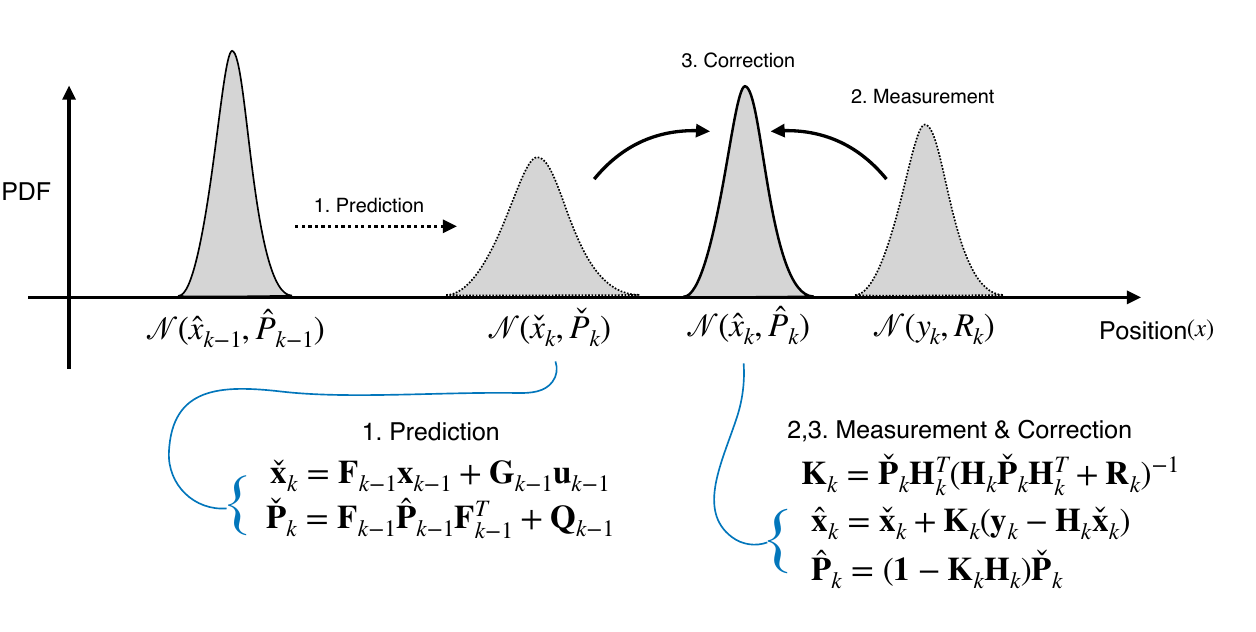
\includegraphics[scale=0.280]{img/kalman_filter/kalman_3.jpeg}
%\end{center}
%\caption{The linear Kalman filter steps.}
%\label{kalman_3}
%\end{figure}


\subsection{Questions}
\label{questions_particle_filters}

\begin{enumerate}
\item Which of the following statements, regarding the usefulness of particle filters, are true?


\begin{enumerate}
\item Particle filters are useful as they can handle almost any models
\item Particle filters are useful as within reasonable computational complexity, the particle filter always gives us the best performance. 
\item Particle filters are useful as they give us a compact description of the posterior density. 
\item Particle filters are useful as they give a non-parametric description of the posterior.
\end{enumerate}
\item Assuming that we describe our posterior using the following approximation
\begin{equation}
p(\mathbf{x}_k | \mathbf{y}_{1:k}) \approx \sum_{i=1}^N w_{k}^{(i)} \delta (\mathbf{x}_k -\mathbf{x}_{k}^{(i)})
\end{equation}

what is the MMSE estimate of $\mathbf{x}_k$?
\begin{enumerate}
\item $\hat{\mathbf{x}}_k = \sum_{i}^{N} w_{k}^{(i)} \mathbf{x}_{k}^{(i)}$
\item $\hat{\mathbf{x}}_k = \mathbf{x}_{k}^{(j)} ~~ \text{where} ~~ j = argmax_i w_{k}^{(i)}$
\item $\hat{\mathbf{x}}_k = \frac{1}{N}\sum_{i}^{N}  \mathbf{x}_{k}^{(i)}$
\item It is not possible to calculate a MMSE estimate from this approximation. 
\end{enumerate}
\item Consider Figure \ref{P0_7_3_4_ex1}.

\begin{figure}[!htb]
\begin{center}
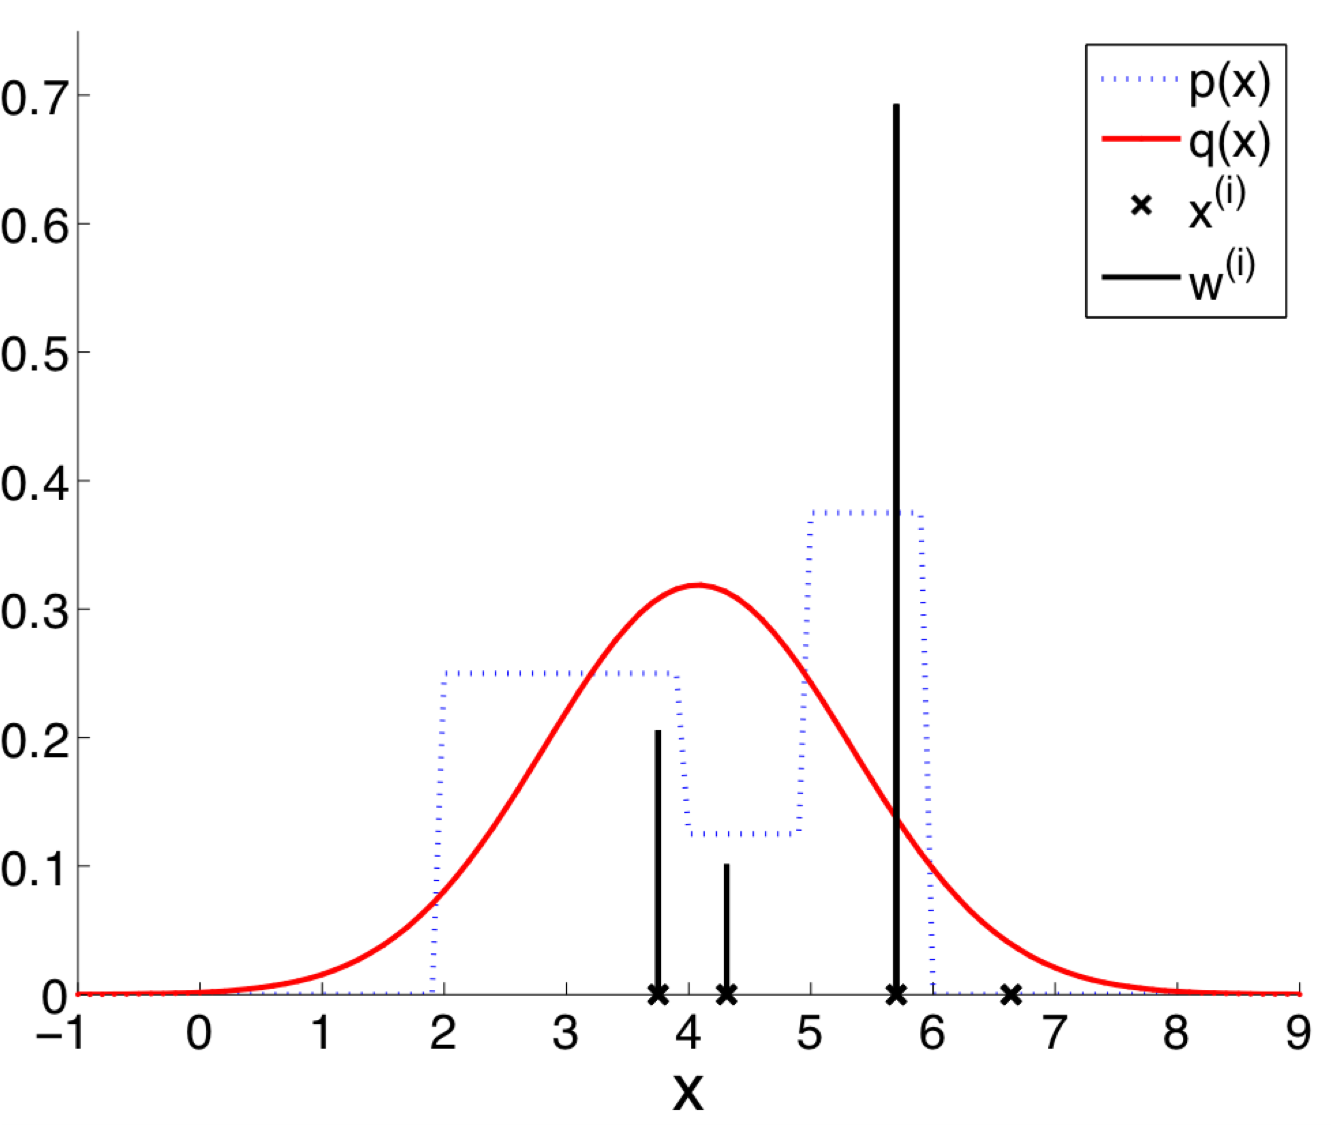
\includegraphics[scale=0.280]{img/particle_filters/P0_7_3_4_ex1.png}
\end{center}
\caption{Question figure.}
\label{P0_7_3_4_ex1}
\end{figure}
Perform resampling on the density and illustrate the result. Assume that the numbers 0.65, 0.03, 0.84 and 0.93 are drawn uniformly from $[0,1]$.
Which one of the following figures illustrates the resampled particles?

\begin{enumerate}
\item \begin{figure}[!htb]
\begin{center}
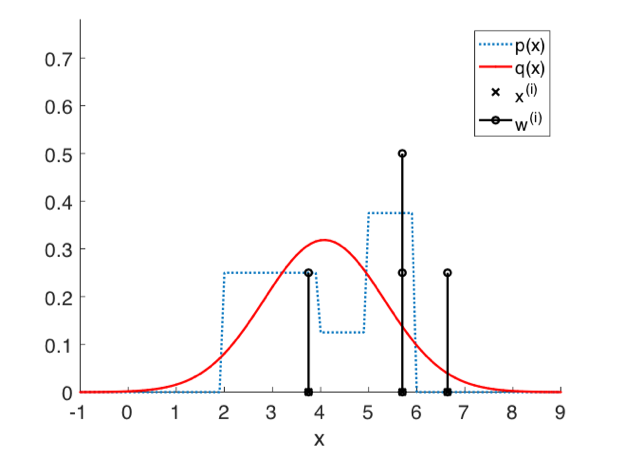
\includegraphics[scale=0.320]{img/particle_filters/P1_7_3_4_ex1.png}
\end{center}
\label{P1_7_3_4_ex1}
\end{figure}
\item \begin{figure}[!htb]
\begin{center}
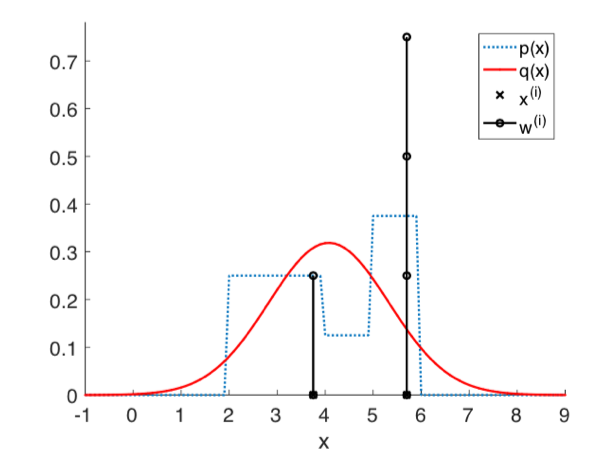
\includegraphics[scale=0.320]{img/particle_filters/P2_7_3_4_ex1.png}
\end{center}
\label{P2_7_3_4_ex1}
\end{figure}
\item \begin{figure}[!htb]
\begin{center}
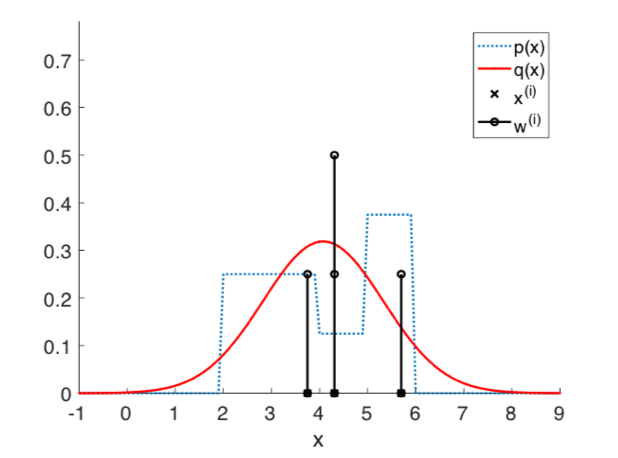
\includegraphics[scale=0.320]{img/particle_filters/P3_7_3_4_ex1.png}
\end{center}
\label{P3_7_3_4_ex1}
\end{figure}
\end{enumerate}

%\begin{figure}
%\begin{subfigure}{.5\textwidth}
%  \centering
%  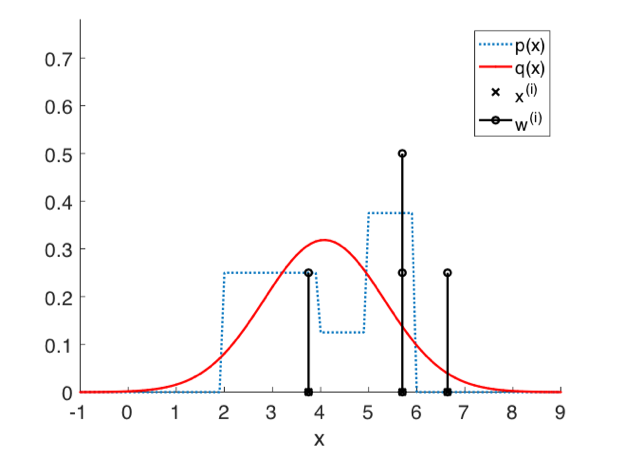
\includegraphics[width=.8\linewidth]{img/particle_filters/P1_7_3_4_ex1.png}
%  \caption{Option A}
%  \label{fig:sfig1}
%\end{subfigure}%
%\begin{subfigure}{.5\textwidth}
%  \centering
%  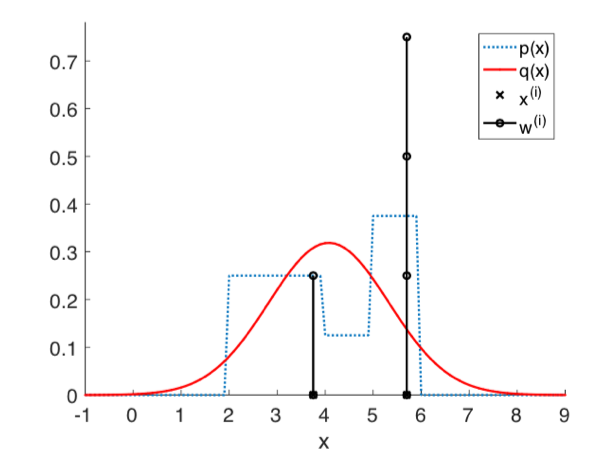
\includegraphics[width=.8\linewidth]{img/particle_filters/P2_7_3_4_ex1.png}
%  \caption{Option B}
%  \label{fig:sfig2}
%\end{subfigure}
%\begin{subfigure}{.5\textwidth}
%  \centering
%  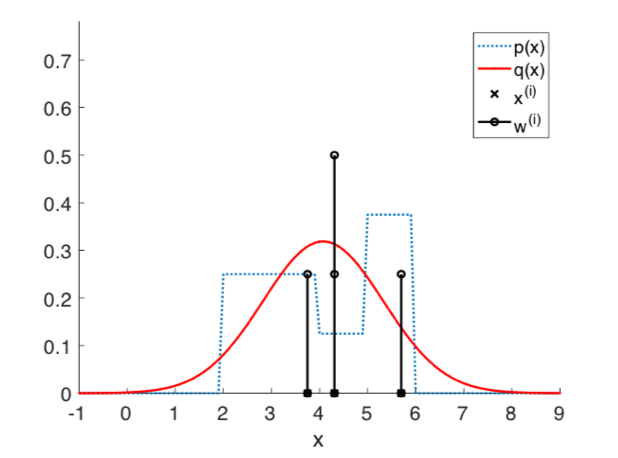
\includegraphics[width=.8\linewidth]{img/particle_filters/P3_7_3_4_ex1.png}
%  \caption{Option C}
%  \label{fig:sfig2}
%\end{subfigure}
%\caption{Options for question.}
%\label{fig:fig}
%\end{figure}

\end{enumerate}




